% called by main.tex
%
\chapter{Resultados}
\label{ch::chapter9}

Todos los resultados presentados en capítulos anteriores han usado el split de validación para desarrollar los modelos, diagnosticar sus fallos y decidir qué variantes
merecía evaluar al final.
En este capítulo se comparan los resultados obtenidos para los mejores modelos de cada familia sobre el conjunto de test.

La comparación mantiene las mismas familias de métricas utilizadas durante el trabajo: parseabilidad del YAML reconstruido, fidelidad del texto de línea, exactitud de
\texttt{level}, adecuación al prompt, cobertura semántica aproximada y validez de dominio Kubernetes.

%----------------------------------------------------------------------
\section{Resultados globales en conjunto test}
\label{sec:ch9_test_results}
%----------------------------------------------------------------------

La Tabla~\ref{tab:ch9_test_results} resume los resultados finales en test. Los porcentajes se expresan sobre 100, salvo \texttt{average\_level\_mae}, que conserva su
escala original.

\begin{table}[htbp]
\centering
\caption{Resultados principales en test. El baseline y THM v1 tienen 62/70, 62/70 ejemplos evaluables respectivamente; \texttt{serialized\_sft}, THOP-FiLM y
las dos variantes DPO tienen 70/70.}
\label{tab:ch9_test_results}
\scriptsize
\resizebox{\textwidth}{!}{%
\begin{tabular}{lrrrrrr}
\toprule
\textbf{Métrica} &
\textbf{Baseline} &
\textbf{\texttt{serialized\_sft}} &
\textbf{THM v1} &
\textbf{THOP-FiLM} &
\textbf{DPO v1} &
\textbf{DPO v2} \\
\midrule
\texttt{yaml\_parse\_success\_rate}       & 46{,}77 & 97{,}14 & 51{,}61 & 31{,}42 & 97{,}14 & 100{,}00 \\
\texttt{average\_line\_text\_f1}          & 31{,}75 & 79{,}09 & 36{,}37 & 16{,}09 & 79{,}46 & 78{,}31 \\
\texttt{average\_level\_exact\_match}     & 22{,}26 & 62{,}98 & 32{,}81 &  5{,}22 & 65{,}05 & 63{,}49 \\
\texttt{average\_level\_mae}              & 0{,}6100 & 0{,}5206 & 0{,}3141 & 1{,}0249 & 0{,}4794 & 0{,}4920 \\
\texttt{average\_prompt\_requirement\_f1} & 32{,}30 & 69{,}32 & 32{,}14 & 13{,}91 & 70{,}35 & 72{,}60 \\
\texttt{average\_semantic\_key\_f1}        & 40{,}82 & 92{,}11 & 46{,}90 & 18{,}82 & 92{,}33 & 94{,}50 \\
\texttt{kubernetes\_domain\_score}        & 38{,}98 & 81{,}67 & 43{,}55 & 14{,}98 & 81{,}67 & 84{,}62 \\
\texttt{kubernetes\_gate\_pass\_rate}     &  8{,}06 & 21{,}43 &  8{,}06 &  1{,}45 & 21{,}43 & 24{,}28 \\
\bottomrule
\end{tabular}
}
\end{table}

La Figura~\ref{fig:ch9_test_metric_heatmap} resume visualmente las mismas cifras para facilitar la comparación entre familias de modelos.

\begin{figure}[htbp]
\centering
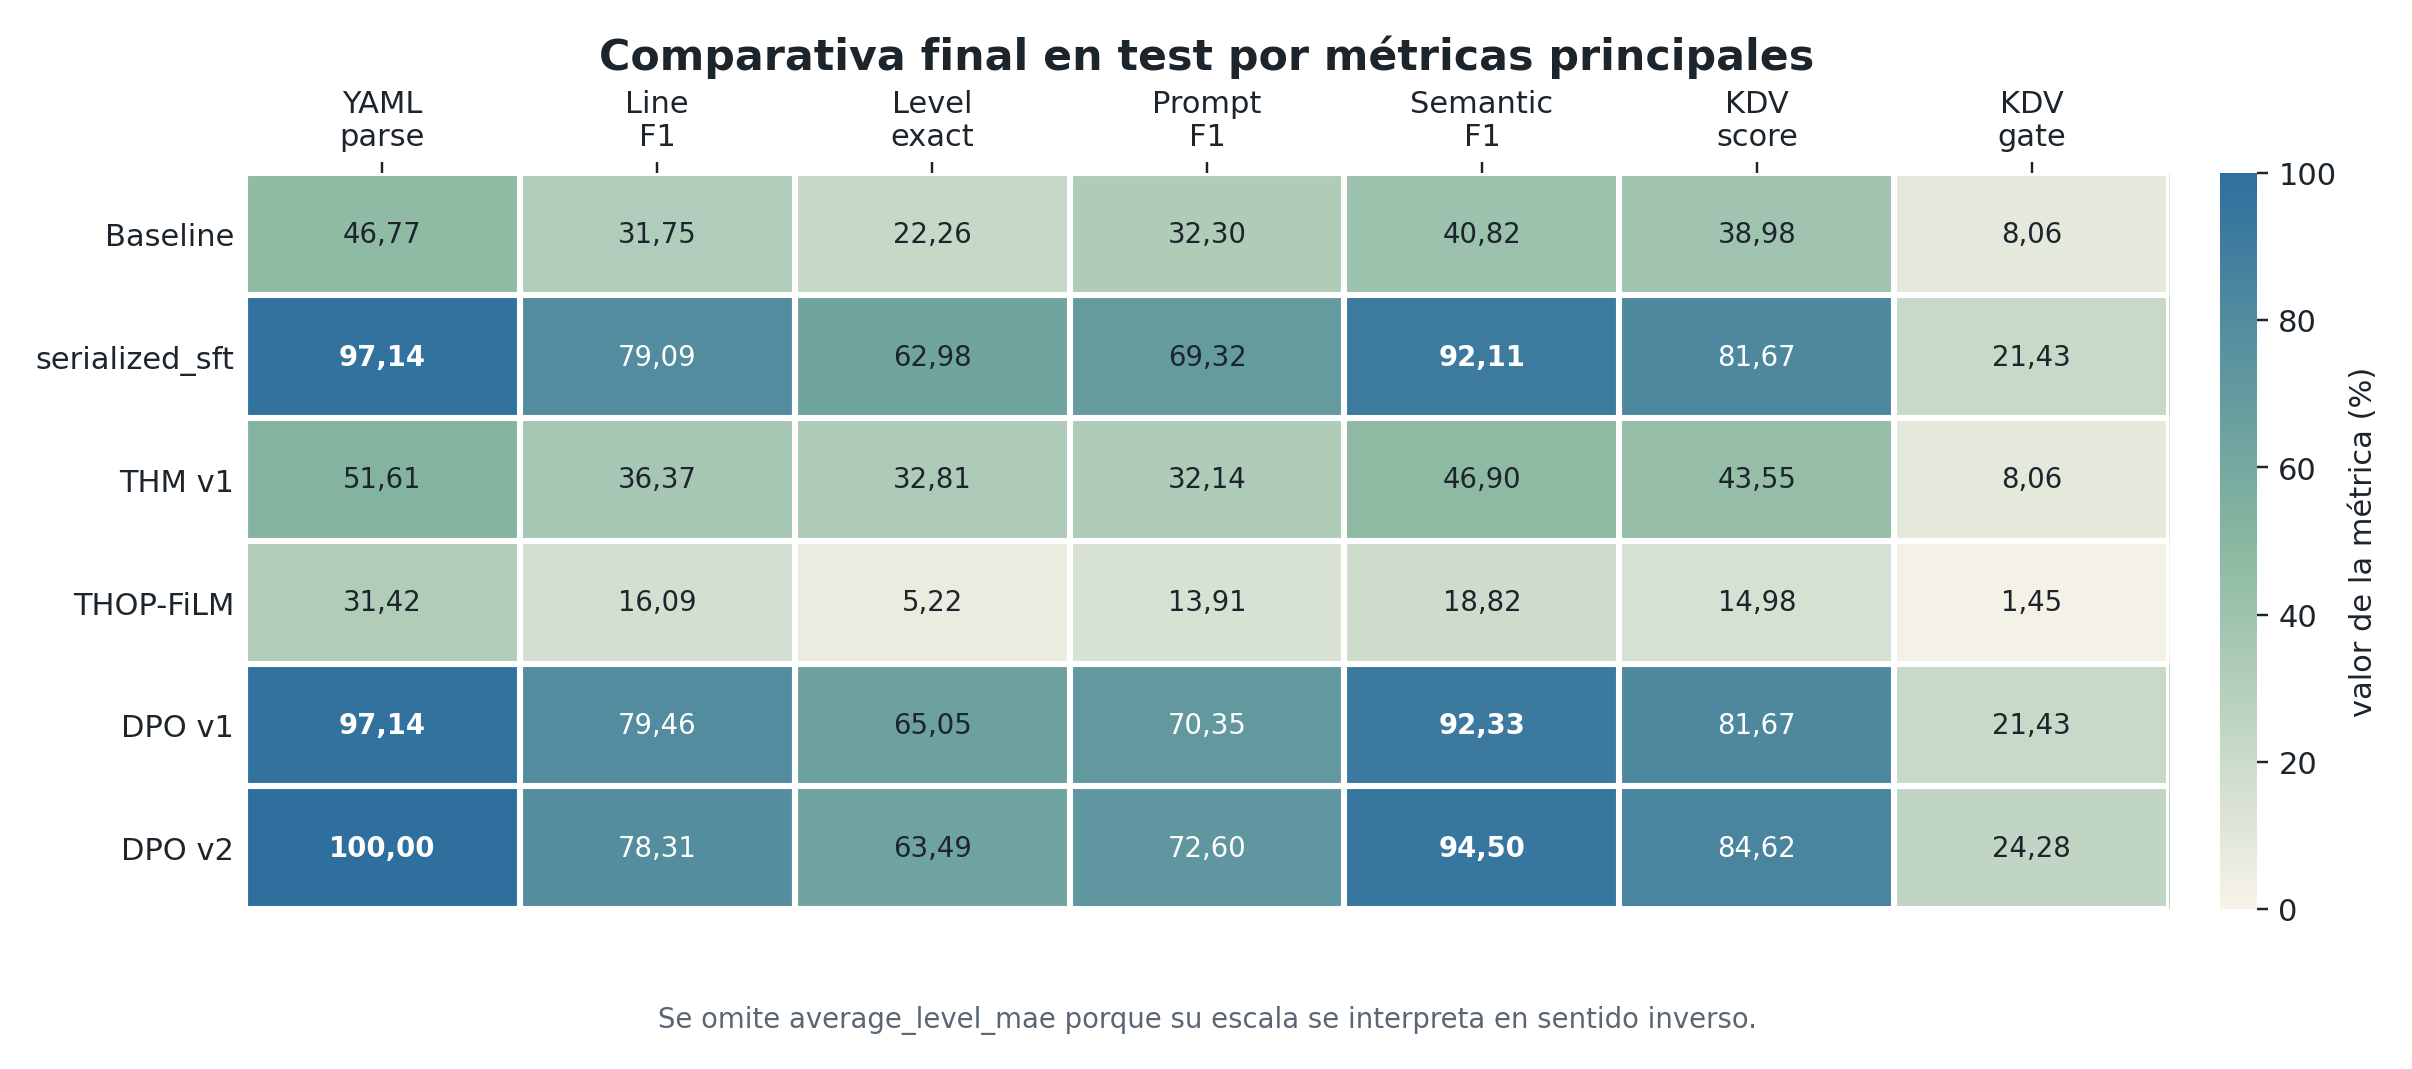
\includegraphics[width=\textwidth]{figures/chapter8/fig8_1_test_metric_heatmap.png}
\caption{Comparativa visual de las métricas principales en test a partir de la Tabla~\ref{tab:ch9_test_results}. Se omite \texttt{average\_level\_mae} porque su escala
se interpreta en sentido inverso: valores menores indican menor error medio de nivel.}
\label{fig:ch9_test_metric_heatmap}
\end{figure}

%----------------------------------------------------------------------
\section{Comentarios sobre la comparación}
\label{sec:ch9_comparison}
%----------------------------------------------------------------------

El salto más claro se produce entre el baseline y el \texttt{serialized\_sft}. El baseline alcanza un 46{,}77\,\% de YAML parseable sobre los ejemplos evaluables,
mientras que el SFT serializado sube hasta el 97{,}14\,\%. La mejora no aparece solo en la sintaxis: el F1 de línea pasa de 31{,}75\,\% a 79{,}09\,\%, la exactitud
de \texttt{level} de 22{,}26\,\% a 62{,}98\,\%, el F1 de requisitos del prompt de 32{,}30\,\% a 69{,}32\,\% y el F1 de claves semánticas de 40{,}82\,\% a 92{,}11\,\%.
En test, por tanto, la serialización supervisada de la jerarquía confirma el mismo cambio de régimen observado durante validación: el modelo deja de limitarse a
producir una superficie reconocible y empieza a generar bloques que el parser puede reconstruir de forma estable.

La comparación con el modelo THM v1 es menos favorable para la hipótesis del cabezal explícito en su forma actual. THM v1 mejora al baseline en parseabilidad
YAML, F1 de línea, exactitud de \texttt{level} y score de dominio, pero queda muy lejos del SFT serializado: 51{,}61\,\% de YAML parseable frente a 97{,}14\,\%, y
36{,}37\,\% de F1 de línea frente a 79{,}09\,\%. El MAE de nivel es menor en THM v1, pero esa ventaja no compensa la pérdida global de parseabilidad y contenido.

THOP-FiLM confirma esta misma lectura. La variante introducía condicionamiento posicional para atacar el problema de los niveles profundos,
pero en test queda en un 31{,}42\,\% de YAML parseable, un 5{,}22\,\% de exactitud de \texttt{level} y un 14{,}98\,\% de score Kubernetes. En este caso, su interés no está en
competir como modelo final, sino en mostrar que añadir posición a una formulación ordinal inestable no basta para recuperar una generación robusta. En términos
de resultados finales, la rama two-head sigue representada de forma más sólida por THM v1.

Las dos variantes DPO se mantienen muy cerca del \texttt{serialized\_sft}. DPO v1 mejora ligeramente el F1 de línea, la exactitud de \texttt{level}, el MAE de nivel
y el F1 de requisitos del prompt, sin cambiar la parseabilidad YAML ni el paso por la compuerta completa de dominio. DPO v2 desplaza algo más el score Kubernetes,
de 81{,}67\,\% a 84{,}62\,\%, alcanza el mejor F1 de requisitos del prompt con 72{,}60\,\% y también el mejor F1 de claves semánticas con 94{,}50\,\%. Además, es
la única variante que llega al 100{,}00\,\% de parseabilidad YAML y eleva la \texttt{kubernetes\_gate\_pass\_rate} hasta el 24{,}28\,\%. Esta mejora viene de la mano
del planteamiento iterativo sobre el dataset, donde la primera versión de las tripletas de entrenamiento se centraba más en la sintaxis, y la segunda versión en
adecuación del prompt y el nivel de completitud de Kubernetes.

La lectura del \textit{gate} completo es especialmente interesante al compararla con las propias referencias del dataset original. Al aplicar la misma compuerta automática
KDV a los YAML esperados, solo el 14{,}29\,\% supera el nivel final. Por tanto, DPO v2 no solo mejora a las demás variantes evaluadas, sino que produce una proporción
mayor de manifiestos que pasan la compuerta automática de buenas prácticas que las propias muestras de referencia del conjunto de test. Esta comparación muestra que la
optimización por preferencias puede desplazar la generación hacia criterios de calidad que no estaban
garantizados en todas las referencias supervisadas.

\begin{figure}[htbp]
\centering
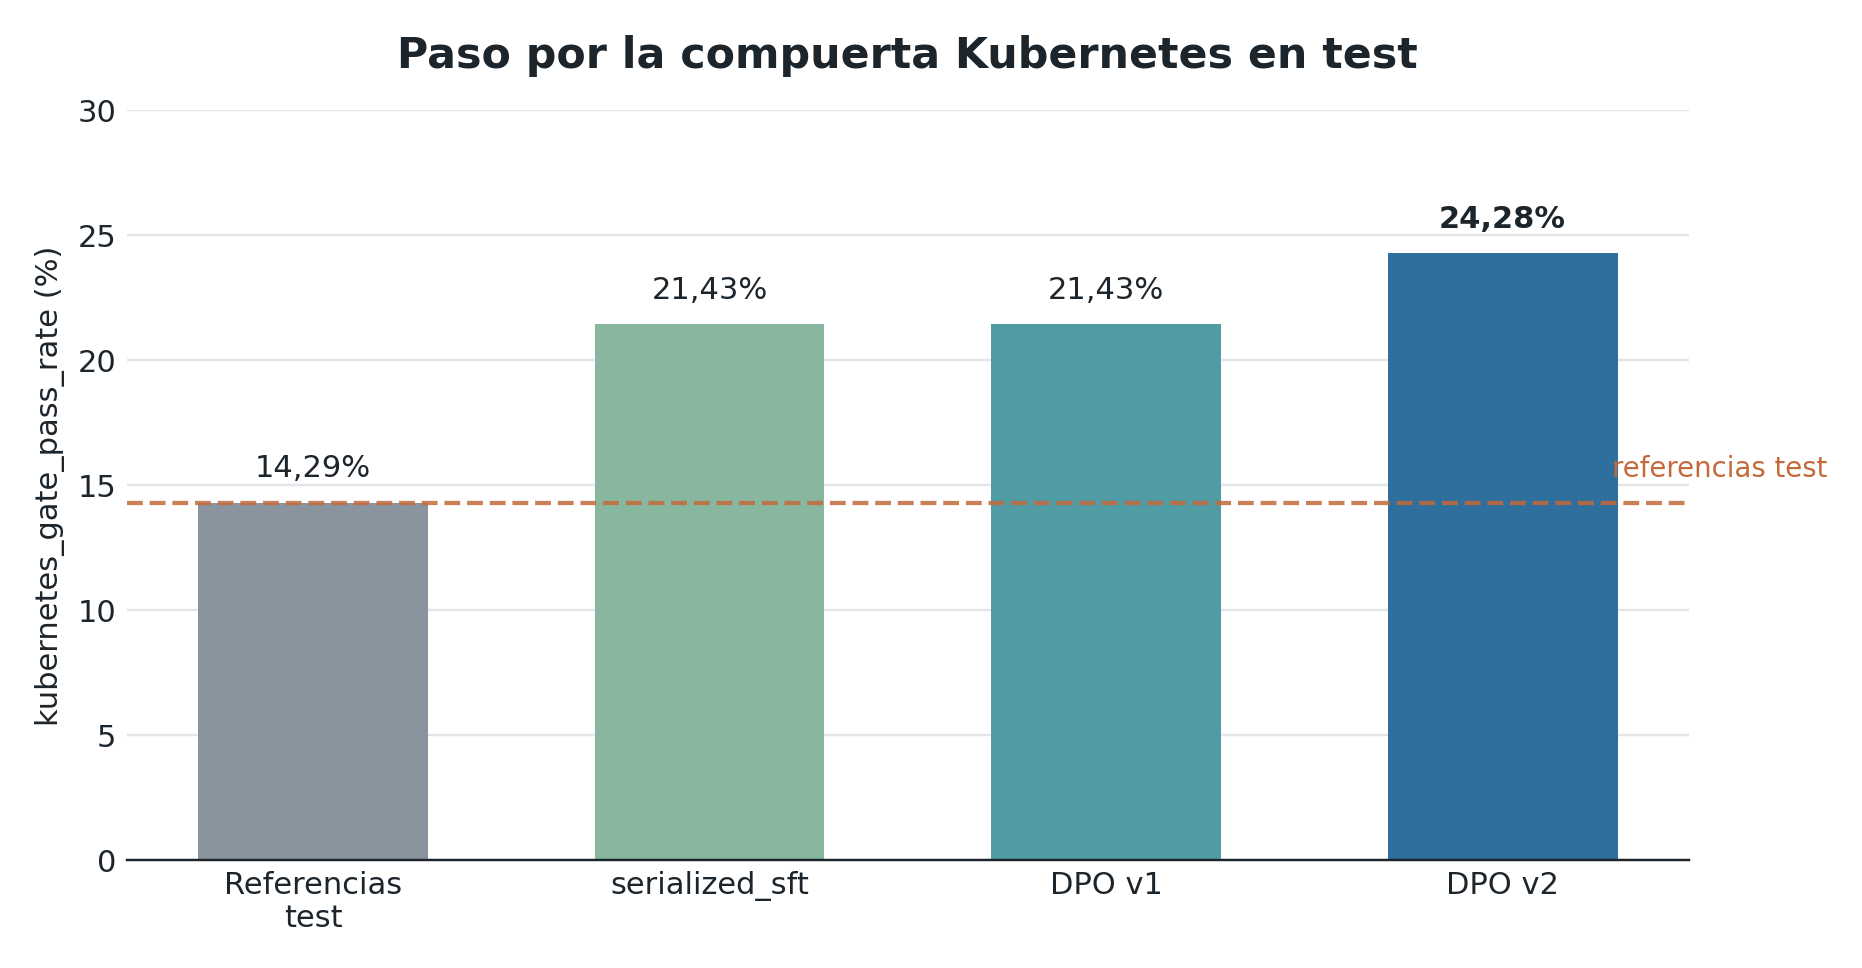
\includegraphics[width=0.78\textwidth]{figures/chapter8/fig8_2_test_gate_reference_comparison.png}
\caption{Comparación de la \texttt{kubernetes\_gate\_pass\_rate} en test entre las referencias del split y las variantes más fuertes de la rama serializada. La compuerta
corresponde al nivel final de la métrica KDV automática}
\label{fig:ch9_test_gate_reference_comparison}
\end{figure}
